\documentclass[a4paper,12pt]{article}

% --- Pacchetti Fondamentali ---
% --- PACCHETTI PER LA MATEMATICA (Mettili qui) ---
\usepackage{amsmath}   % Il pacchetto principale per formule e simboli
\usepackage{amsfonts}  % Per i font matematici come i numeri reali \mathbb{R}
\usepackage{amssymb}   % Per simboli matematici aggiuntivi
\usepackage[utf8]{inputenc} % Codifica caratteri
\usepackage[T1]{fontenc}    % Codifica font
\usepackage[italian]{babel} % Lingua italiana
\usepackage{geometry}       % Gestione margini
\geometry{a4paper, margin=2.5cm}

% --- Pacchetti Matematica e Fisica ---
\usepackage{amsmath, amssymb} % Simboli matematici
\usepackage{siunitx}          % Gestione unità di misura e numeri (FONDAMENTALE)
\sisetup{
    output-decimal-marker = {.}, % Punto come separatore decimale
    separate-uncertainty = true, % Scrive errori come (Valore +/- Errore)
    per-mode = symbol            % Usa / per le unità (m/s)
}

% --- Pacchetti Immagini e Tabelle ---
\usepackage{graphicx} % Per inserire PNG/JPG
\usepackage{float}    % Per forzare la posizione delle immagini (H)
\usepackage{booktabs} % Per tabelle professionali (\toprule, \midrule)
\usepackage[justification=centering]{caption}  % Per personalizzare le didascalie
\usepackage{subcaption}

% --- Dati Intestazione ---
\title{\textbf{Risposta dielettrica in radiazione polarizzata a singola lunghezza d'onda}}
\author{Filippo Audisio, Cataldo Insalaco, Telemaco Pezzoni}
\date{\today}

\begin{document}

    \maketitle

    % -------------------------------------------------------------------
    \section{Obiettivo dell'esperienza}
    
    L'obbiettivo di questa esperienza consiste nella misura, per materiali di tipologie differenti, della risposta dielettrica in riflessione e trasmissione a lunghezza d'onda prescelta con luce polarizzata. Nello specifico si vuole:
    \begin{itemize}
        \item Determinare l'andamento angolare di $T_s$ e $T_p$ per $SiO_2$, $R_s$ e $R_p$ per $SiO_2$ e $Si$; poi trovare il valore dell'angolo di Brewster per entrambi i materiali
        \item Stimare il valore dell'indice di rifrazione per entrambi i materiali ed il grado di polarizzazione in $R$
    \end{itemize}
    % -------------------------------------------------------------------
    \section{Materiali e Metodi}

    \begin{itemize}
    \item LED verde, alimentato in onda quadra a $1$\unit{kHz}
    \item Lente accoppiata al LED
    \item Tripletto di lenti per focalizzazione.
    \item Polarizzatore lineare Thorlabs LPVISE2X2, banda $400-700$\unit{nm}
    \item Goniometro $\theta$-$2\theta$ solidale al banco di lavoro
    \item Portacampioni.
    \item Fotodiodo in Si polarizzato in inversa, con carico di $10/47$ \unit{k\Omega}
    \item Multimetro
    \item Campioni: vetro amorfo in $SiO_2$ spesso $1$\unit{mm}, $Si$ cristallino spesso $0.5$\unit{mm}
    \item Generatore di funzioni
    \end{itemize}
 
\subsection{Procedura sperimentale}
Per prima cosa si alimenta il LED verde collegandolo al generatore di funzioni con un'onda quadra a $1$\unit{kHz}. Dopodiché si passa all'allineamento del sistema, variando la posizione delle varie componenti fino a massimizzare il segnale rivelato in aria, per poi inserire il polarizzatore a $0$\unit{deg} $90$\unit{deg} così da misurare le intensità iniziali $I_0^s$ e $I_0^p$.
Una volta inserito il campione di vetro si effettuano le misure in trasmisisone, ruotando progressivamente di $5$\unit{deg} il campione e normalizzando i valori rivelati all'intensità misurata inizialmente; il procedimento viene ripetuto per polarizzazione s e p.
In seguito si passa in configurazione di riflessione, allineando con il braccio più lungo il rivelatore all'angolo 2$\theta$ e si agisce sul posizionamento del campione ruotandolo in un intorno di $\theta$ fino a massimizzare il segnale riflesso; anche in questo caso la misura viene ripetuta per entrambe le tipologie di polarizzazione.
Infine nella stessa configurazione si acquisiscono le misure in riflessione del campione di $Si$.
\begin{figure}[H]
     \centering
     \begin{subfigure}[b]{0.45\textwidth}
         \centering
         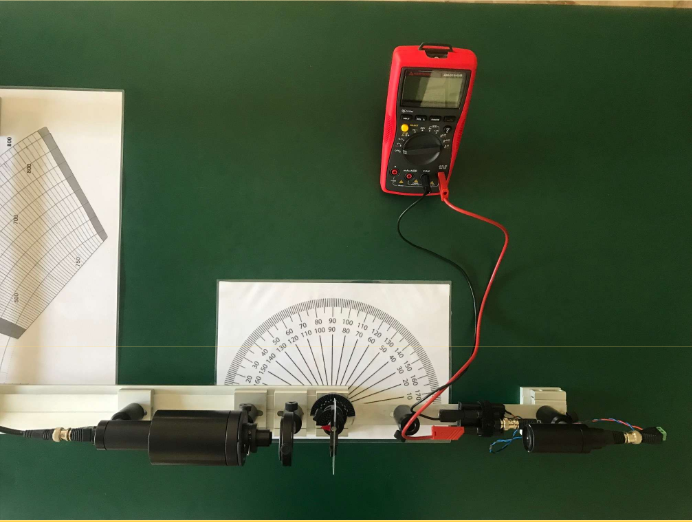
\includegraphics[width=\textwidth]{configurazione_trasmissione.png}
         \subcaption{Configurazione di trasmissione.}
         \label{fig:1a}
     \end{subfigure}
     \begin{subfigure}[b]{0.45\textwidth}
         \centering
         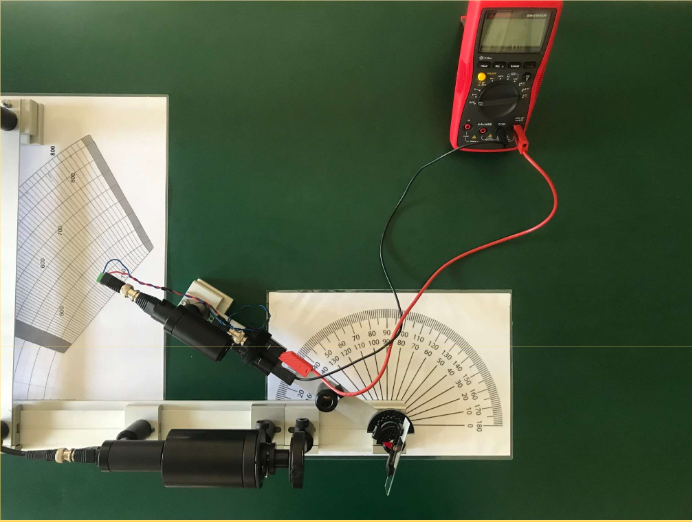
\includegraphics[width=\textwidth]{configurazione_riflessione.png}
         \subcaption{Configurazione di riflessione.}
         \label{fig:1b}
     \end{subfigure}
\end{figure}

\section{Dati sperimentali e Analisi}
\subsection{Distribuzione angolare}
Sugli dati acquisiti è stato eseguito un fit sfruttando le formule dei coefficienti di Fresnel.

\begin{figure}[H]
    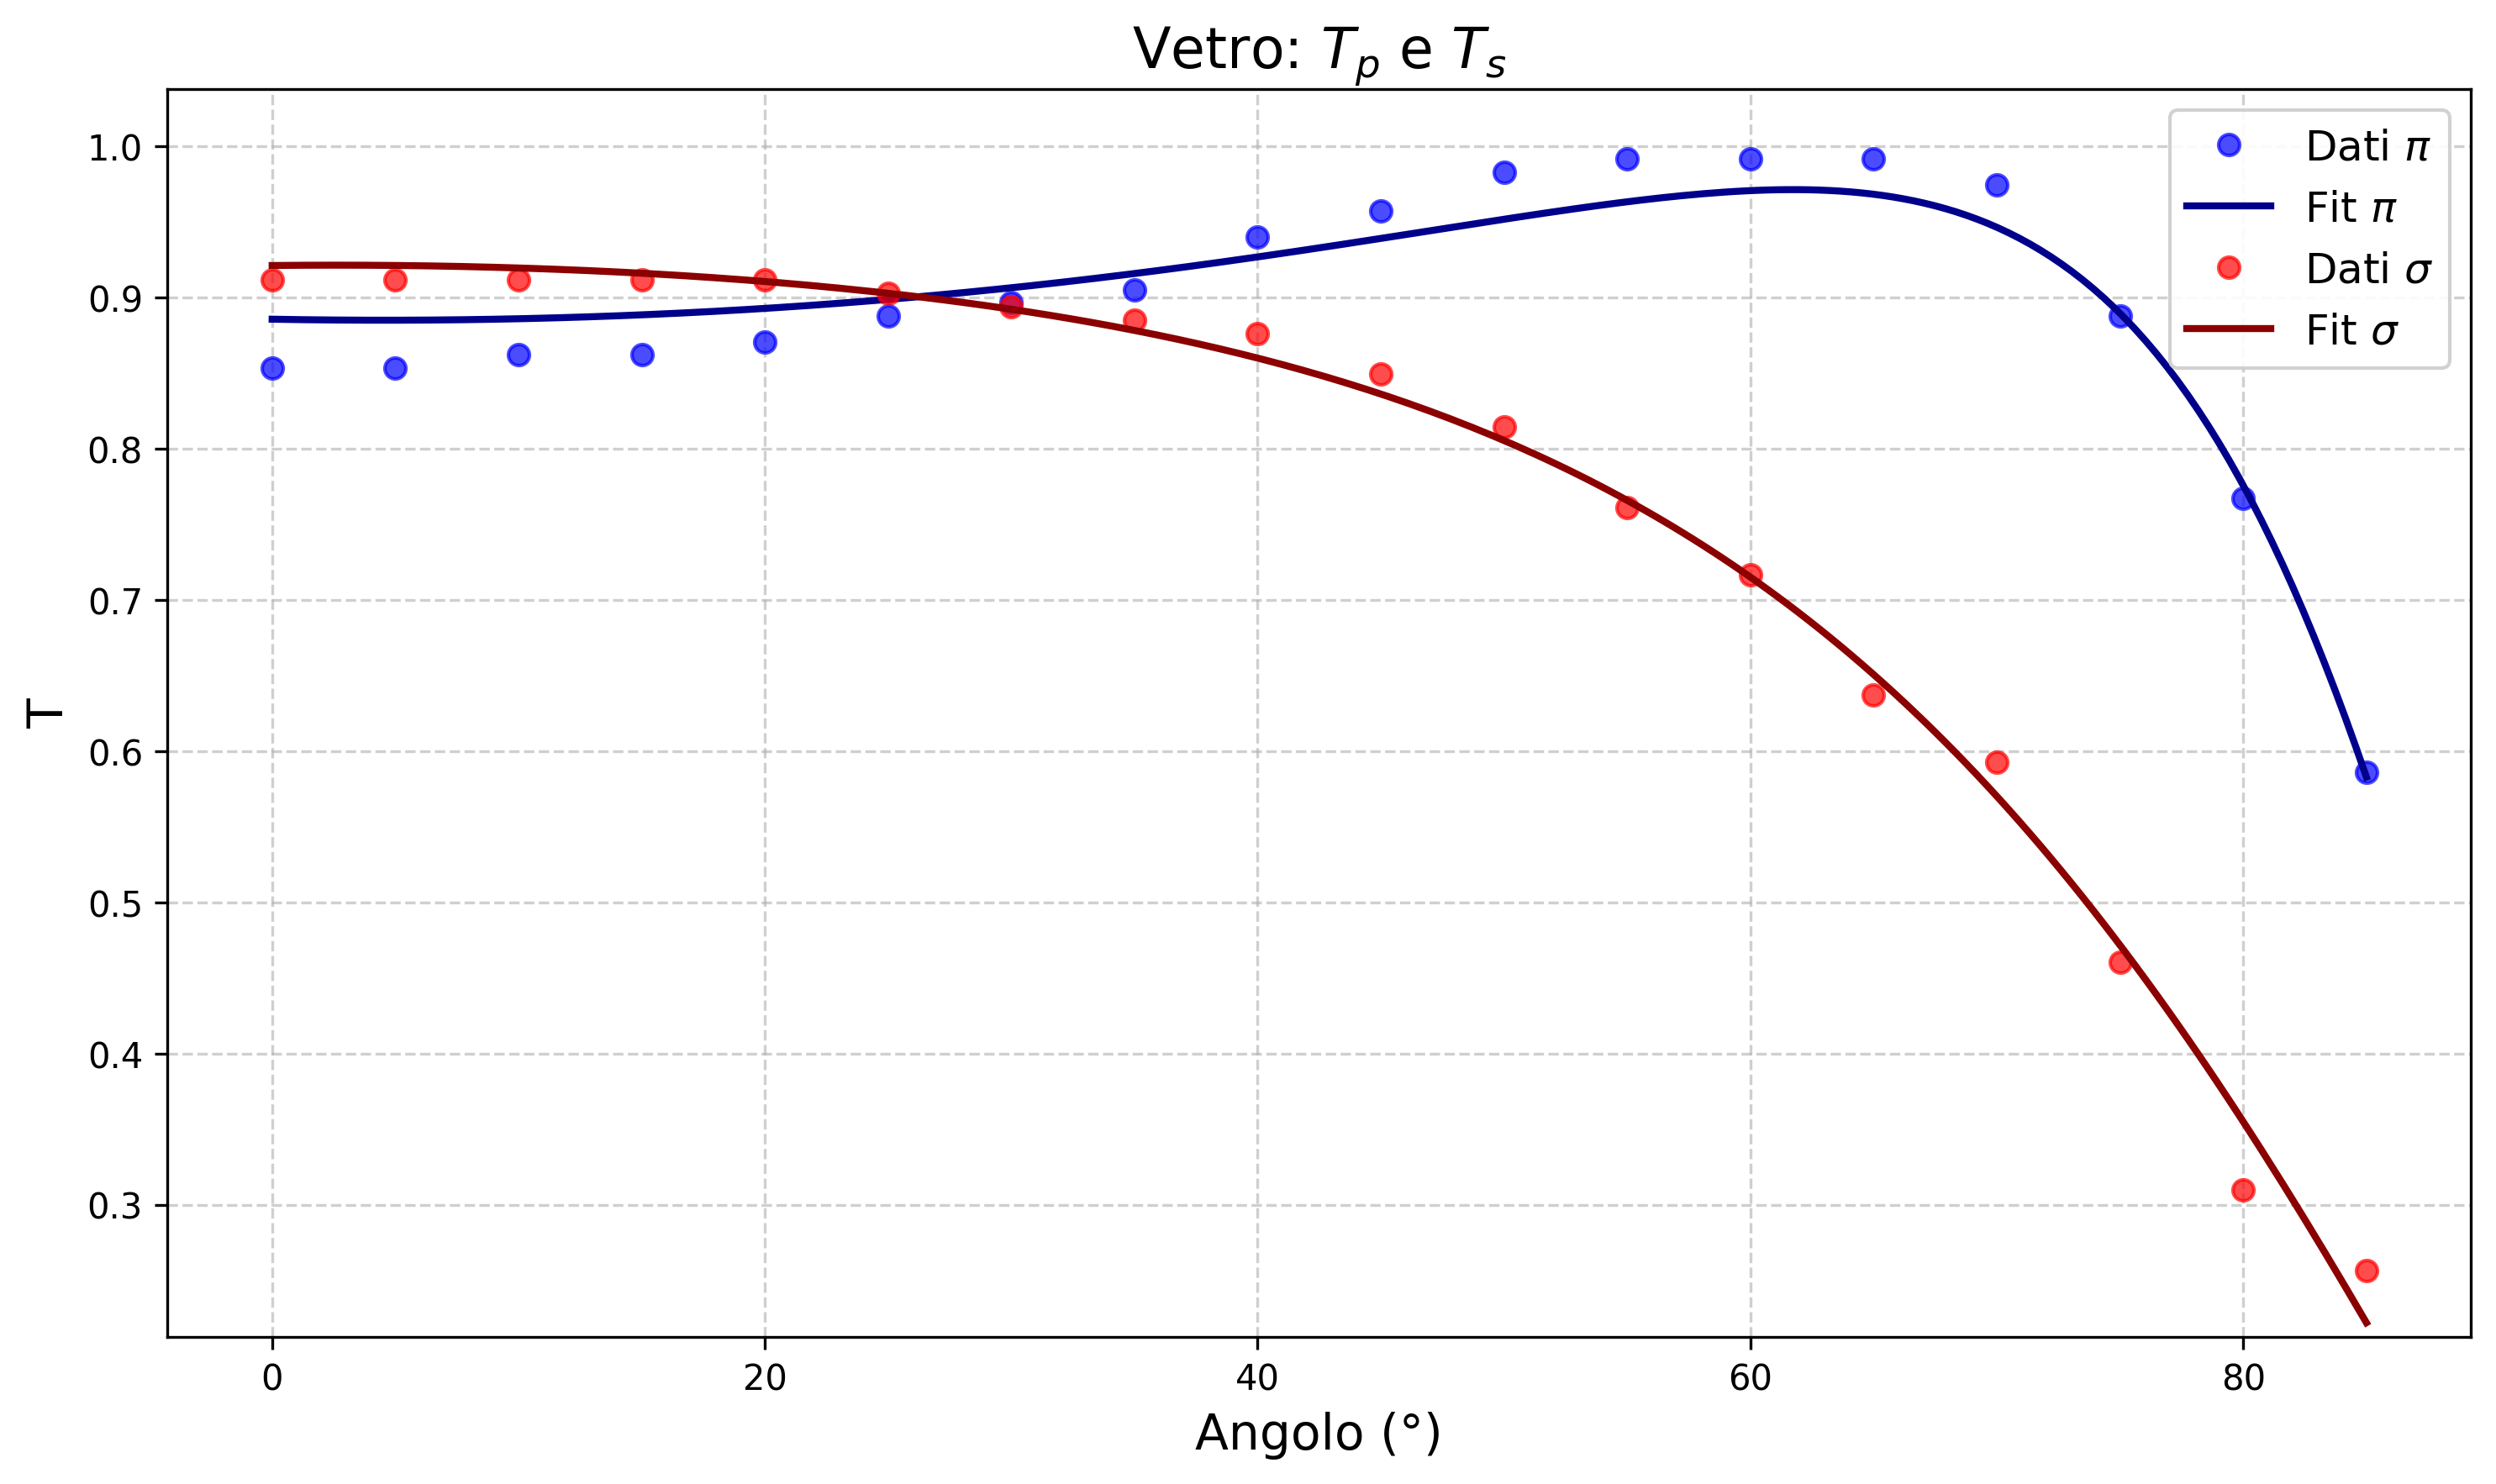
\includegraphics[width=\textwidth]{Combinato_Vetro_T_p_e_T_s.png}
    \caption{Trasmittività Vetro in polarizzazione $\pi$ e $\sigma$}
\end{figure}

\begin{figure}[H]
    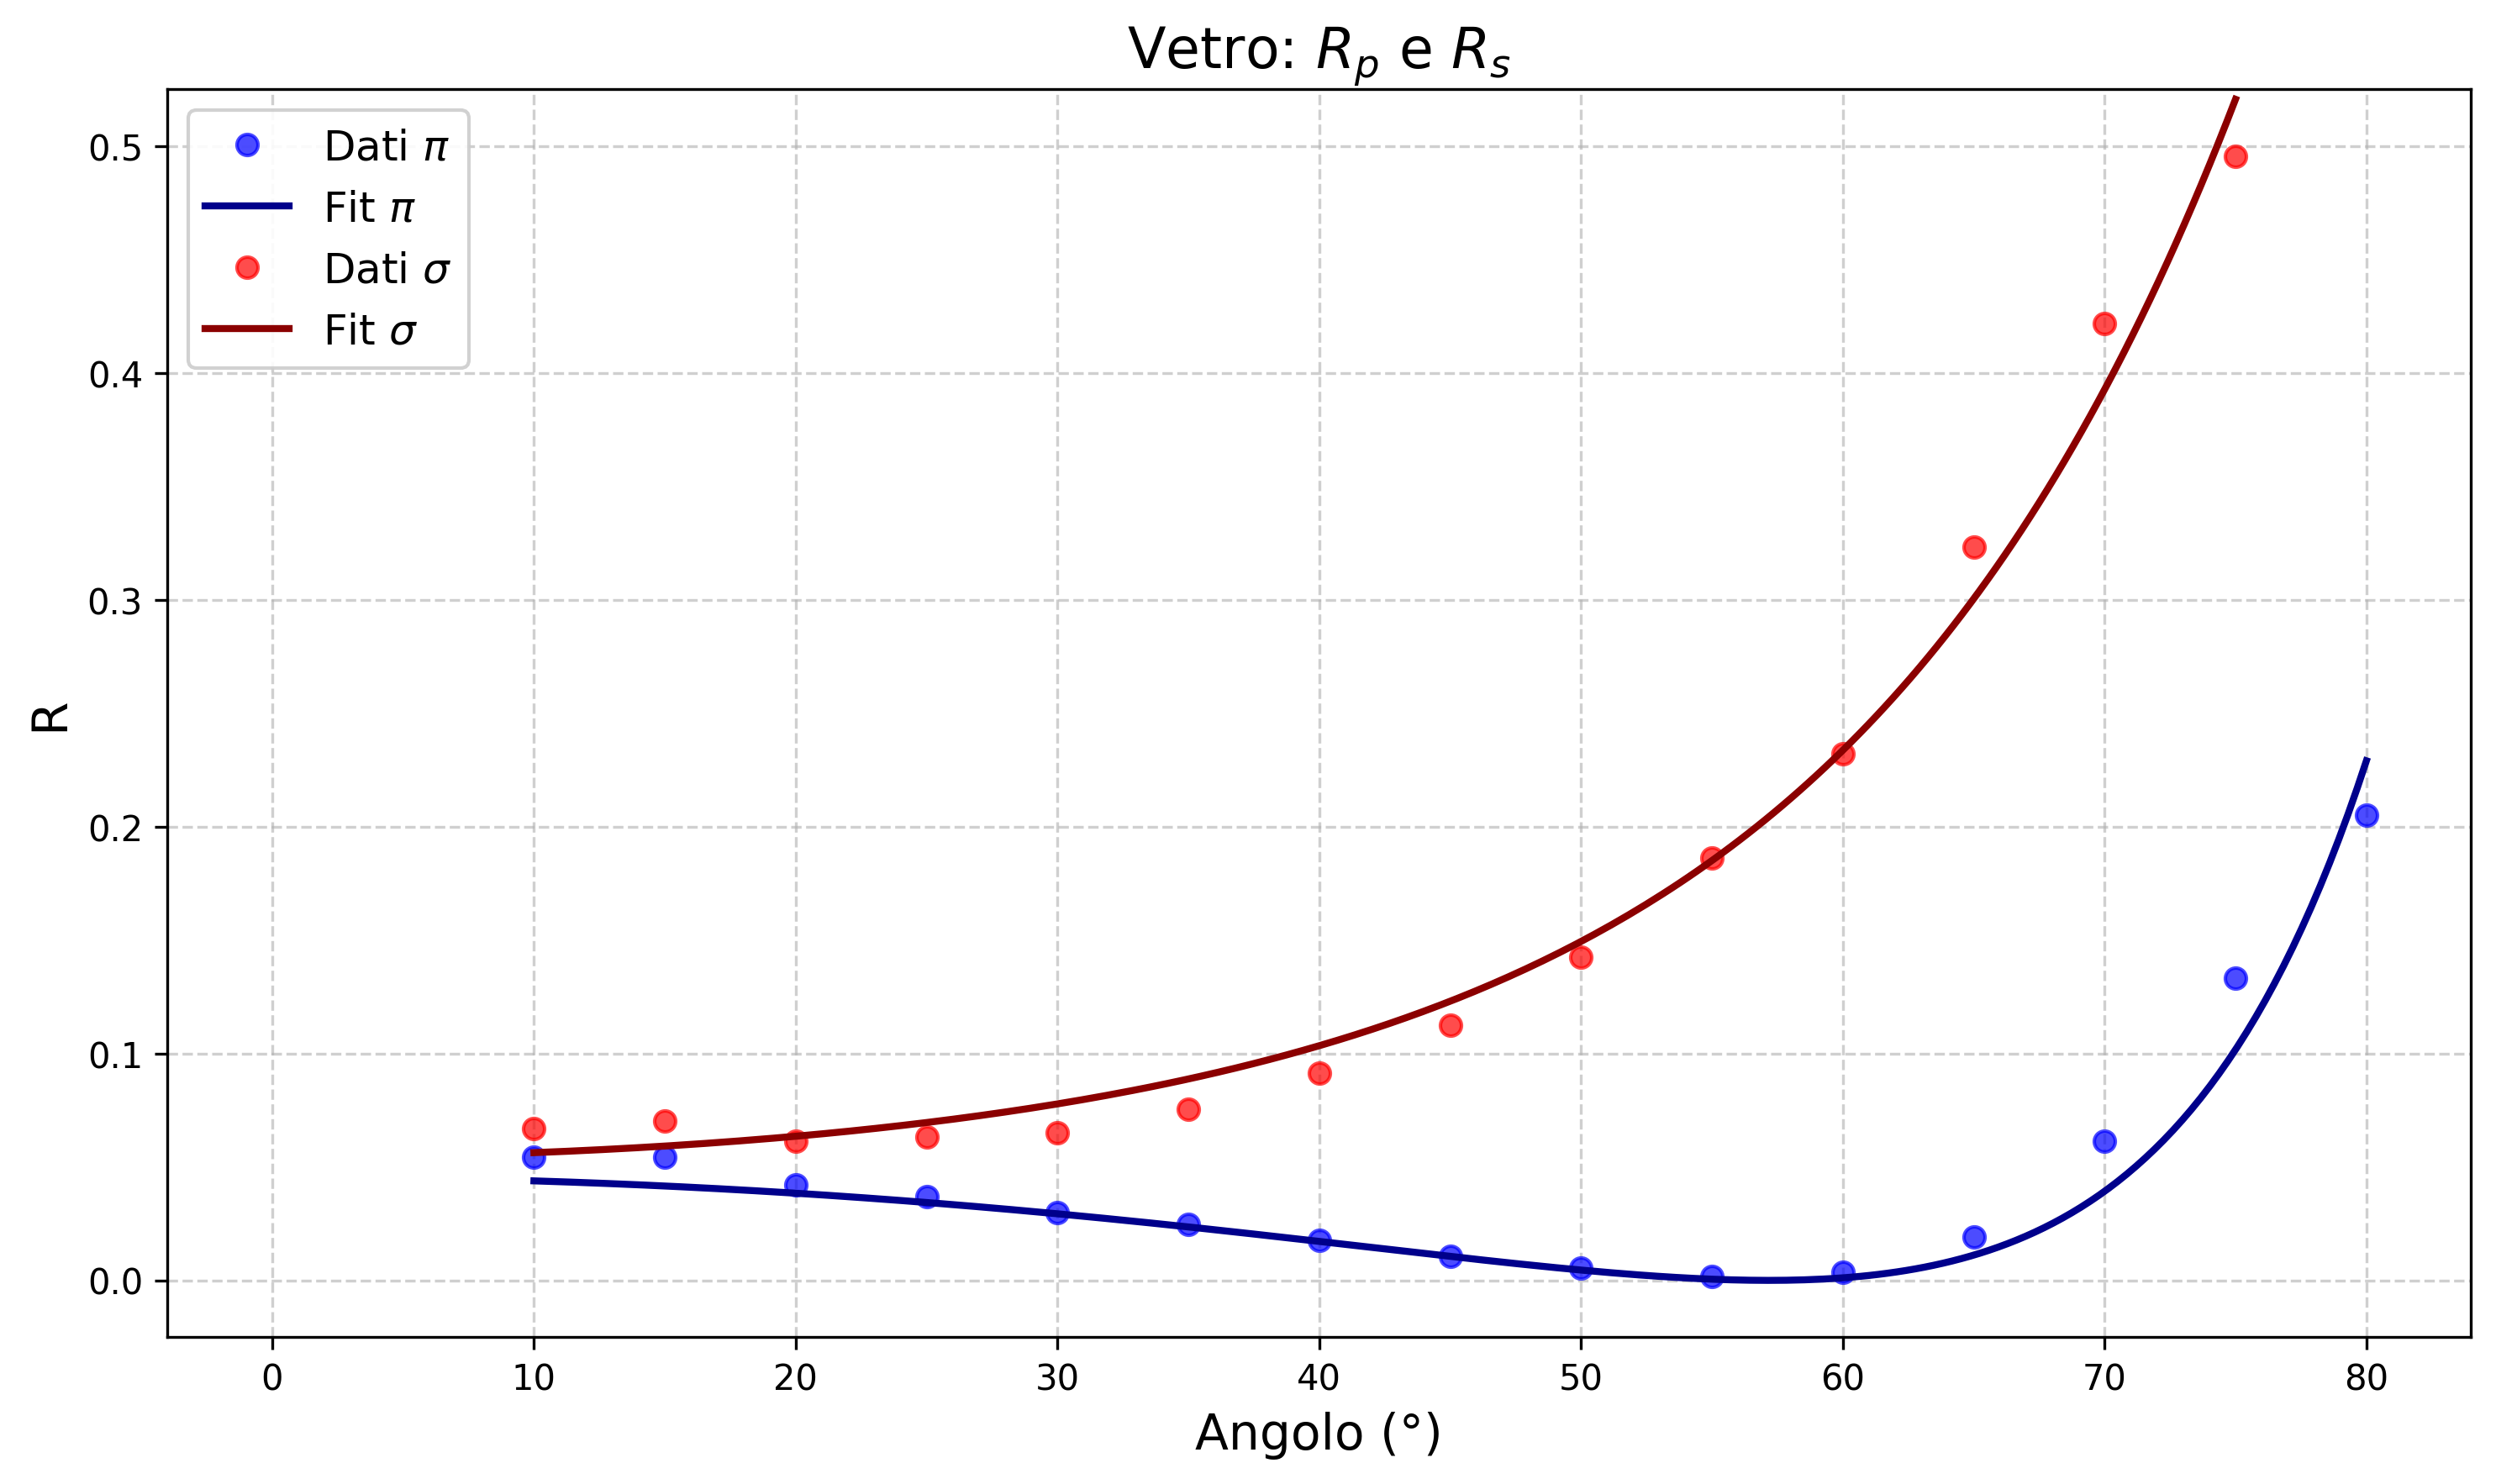
\includegraphics[width=\textwidth]{Combinato_Vetro_R_p_e_R_s.png}
    \caption{Riflettività Vetro in polarizzazione $\pi$ e $\sigma$}
\end{figure}

\begin{figure}[H]
    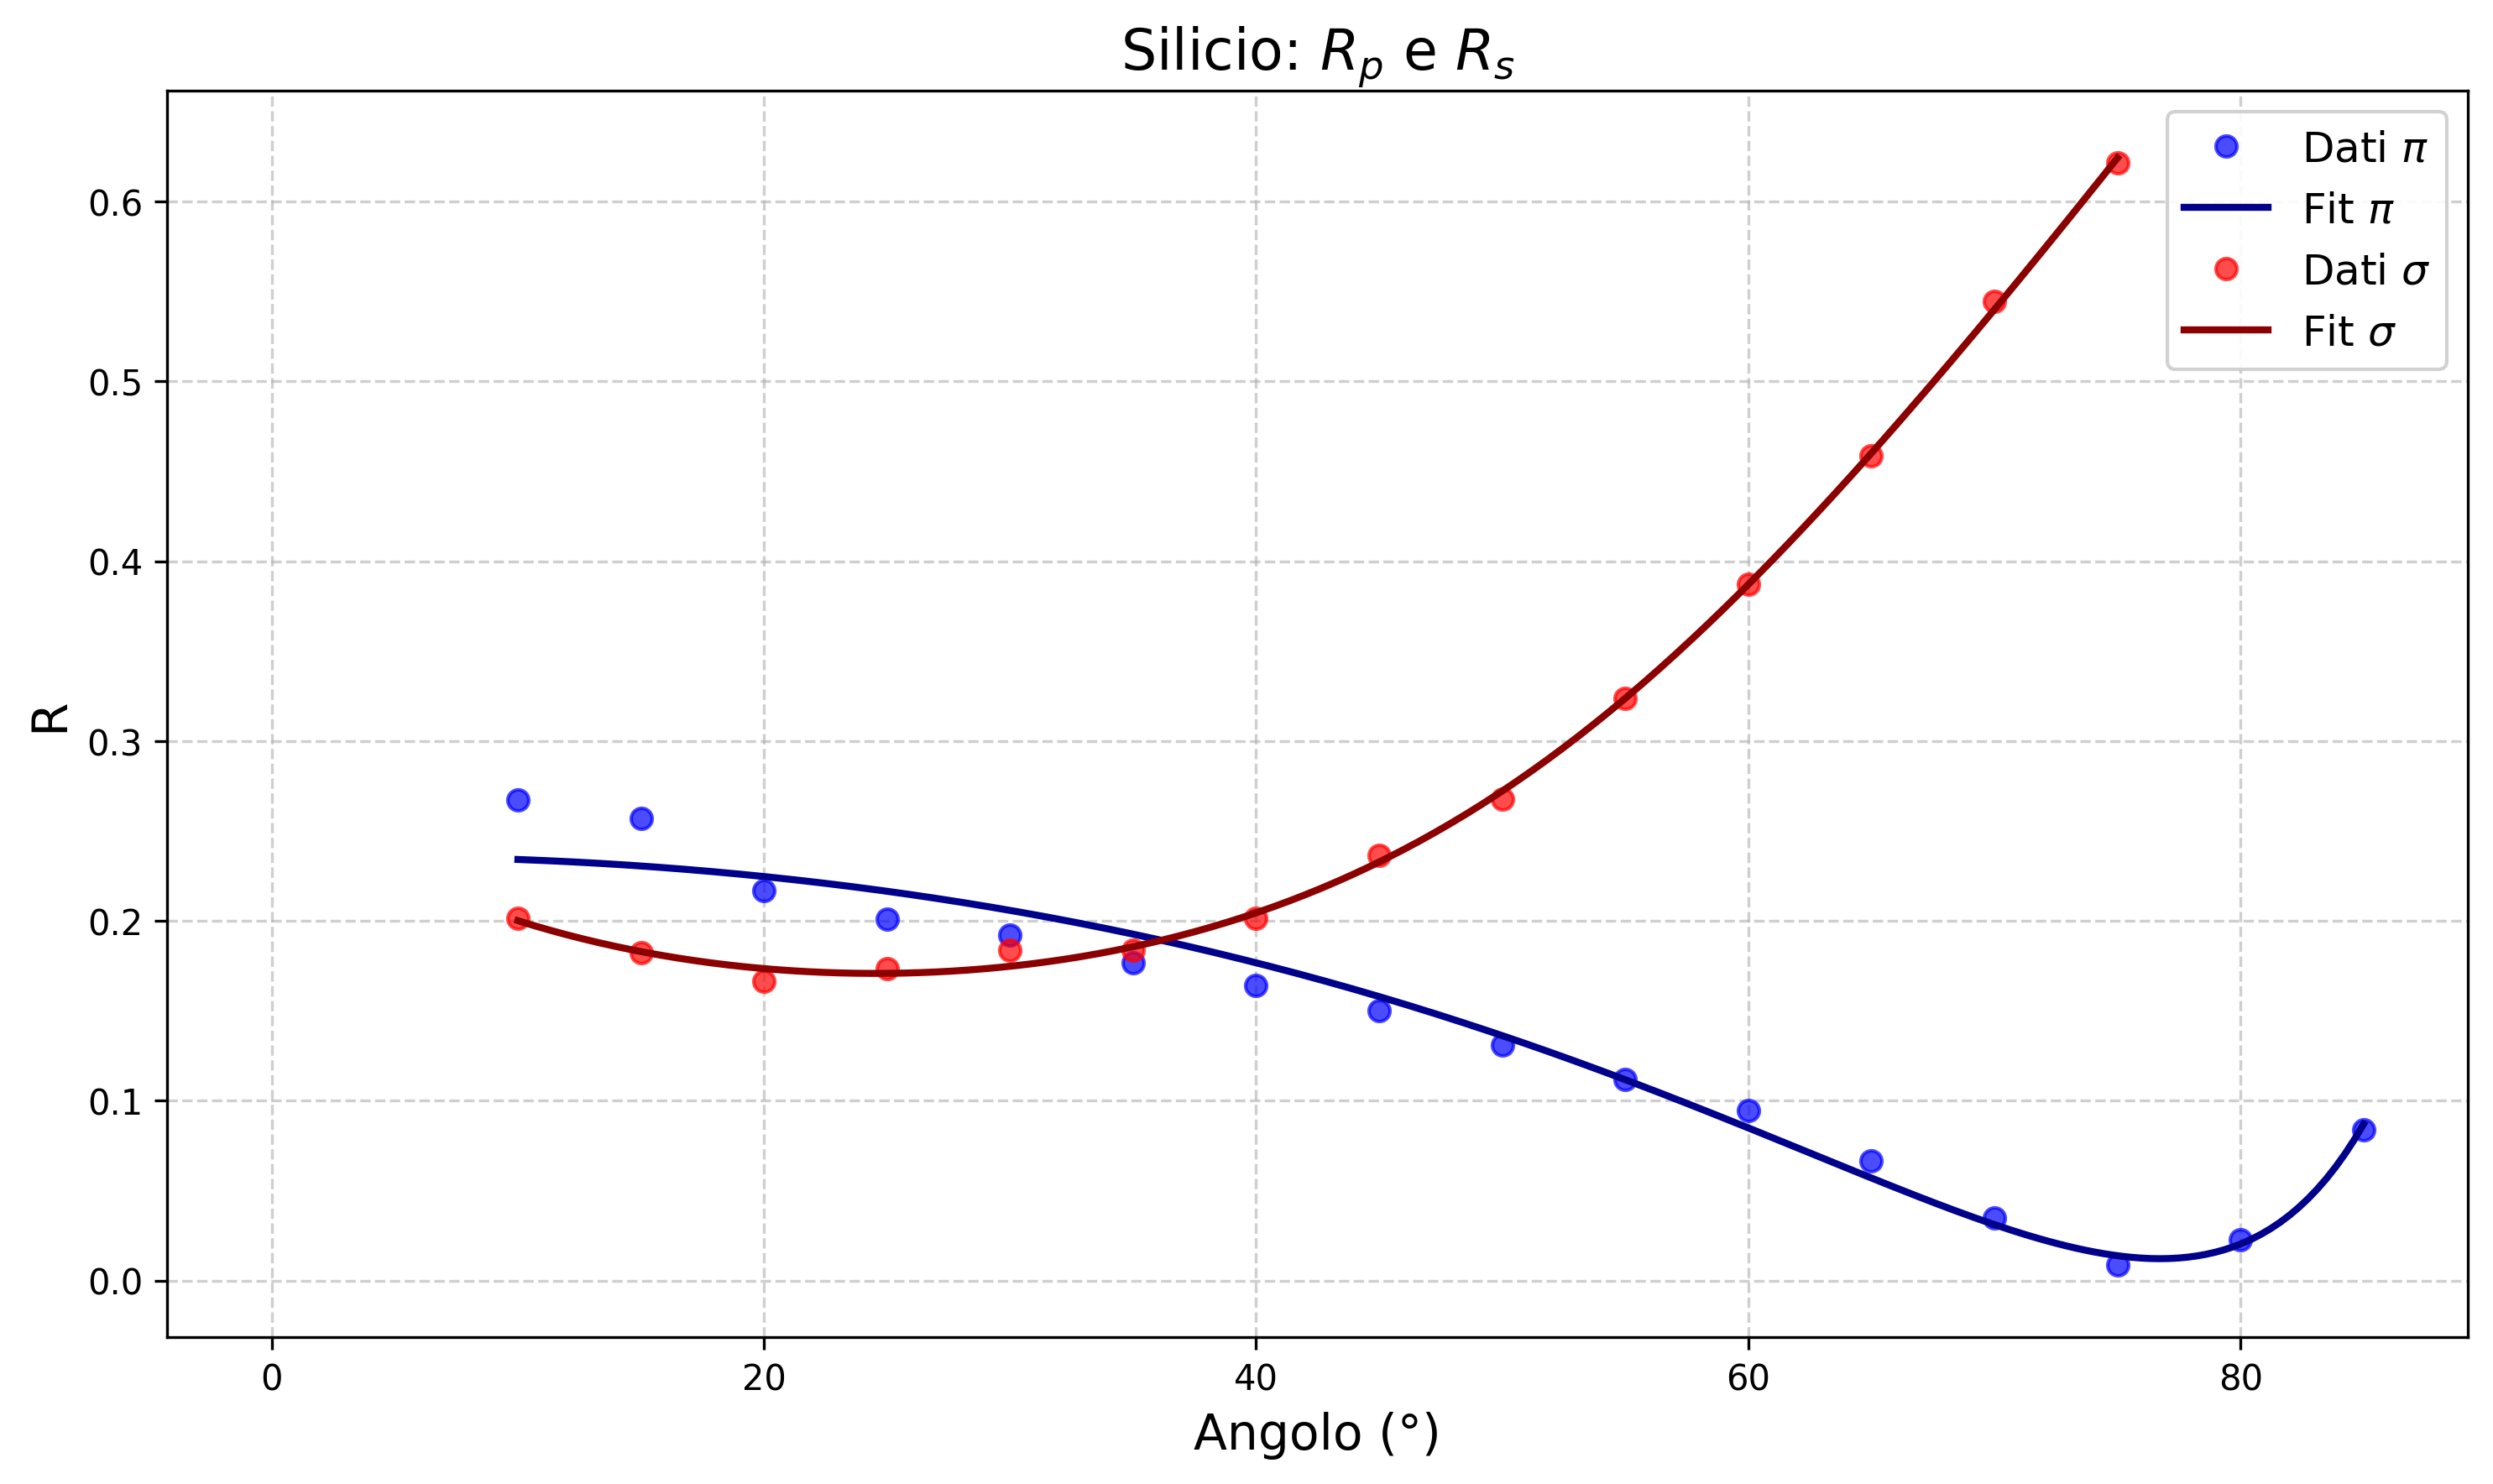
\includegraphics[width=\textwidth]{Combinato_Silicio_R_p_e_R_s.png}
    \caption{Riflettività Silicio in polarizzazione $\pi$ e $\sigma$}
\end{figure}

\begin{table}[H]
    \centering
    \begin{tabular}{
        l
        l
    }
        \toprule
        Campione & $\theta_B$ \\
        \midrule
        $SiO_2$ & $\sim 57$\unit{\degree} \\
        $Si$ & $\sim 76$\unit{\degree} \\
        \bottomrule
    \end{tabular}
    \caption{Angoli di Brewster ricavati dalle distribuzioni angolari}
\end{table}

\subsection{Indice di rifrazione e grado di polarizzazione}
Per ciascun materiale il grado di polarizzazione è stato calcolato sfruttando la formula:
\begin{equation}
    P = \frac{R_s-R_p}{R_s+R_p}
\end{equation}

\begin{figure}[H]
     \centering
     \begin{subfigure}[b]{0.45\textwidth}
         \centering
         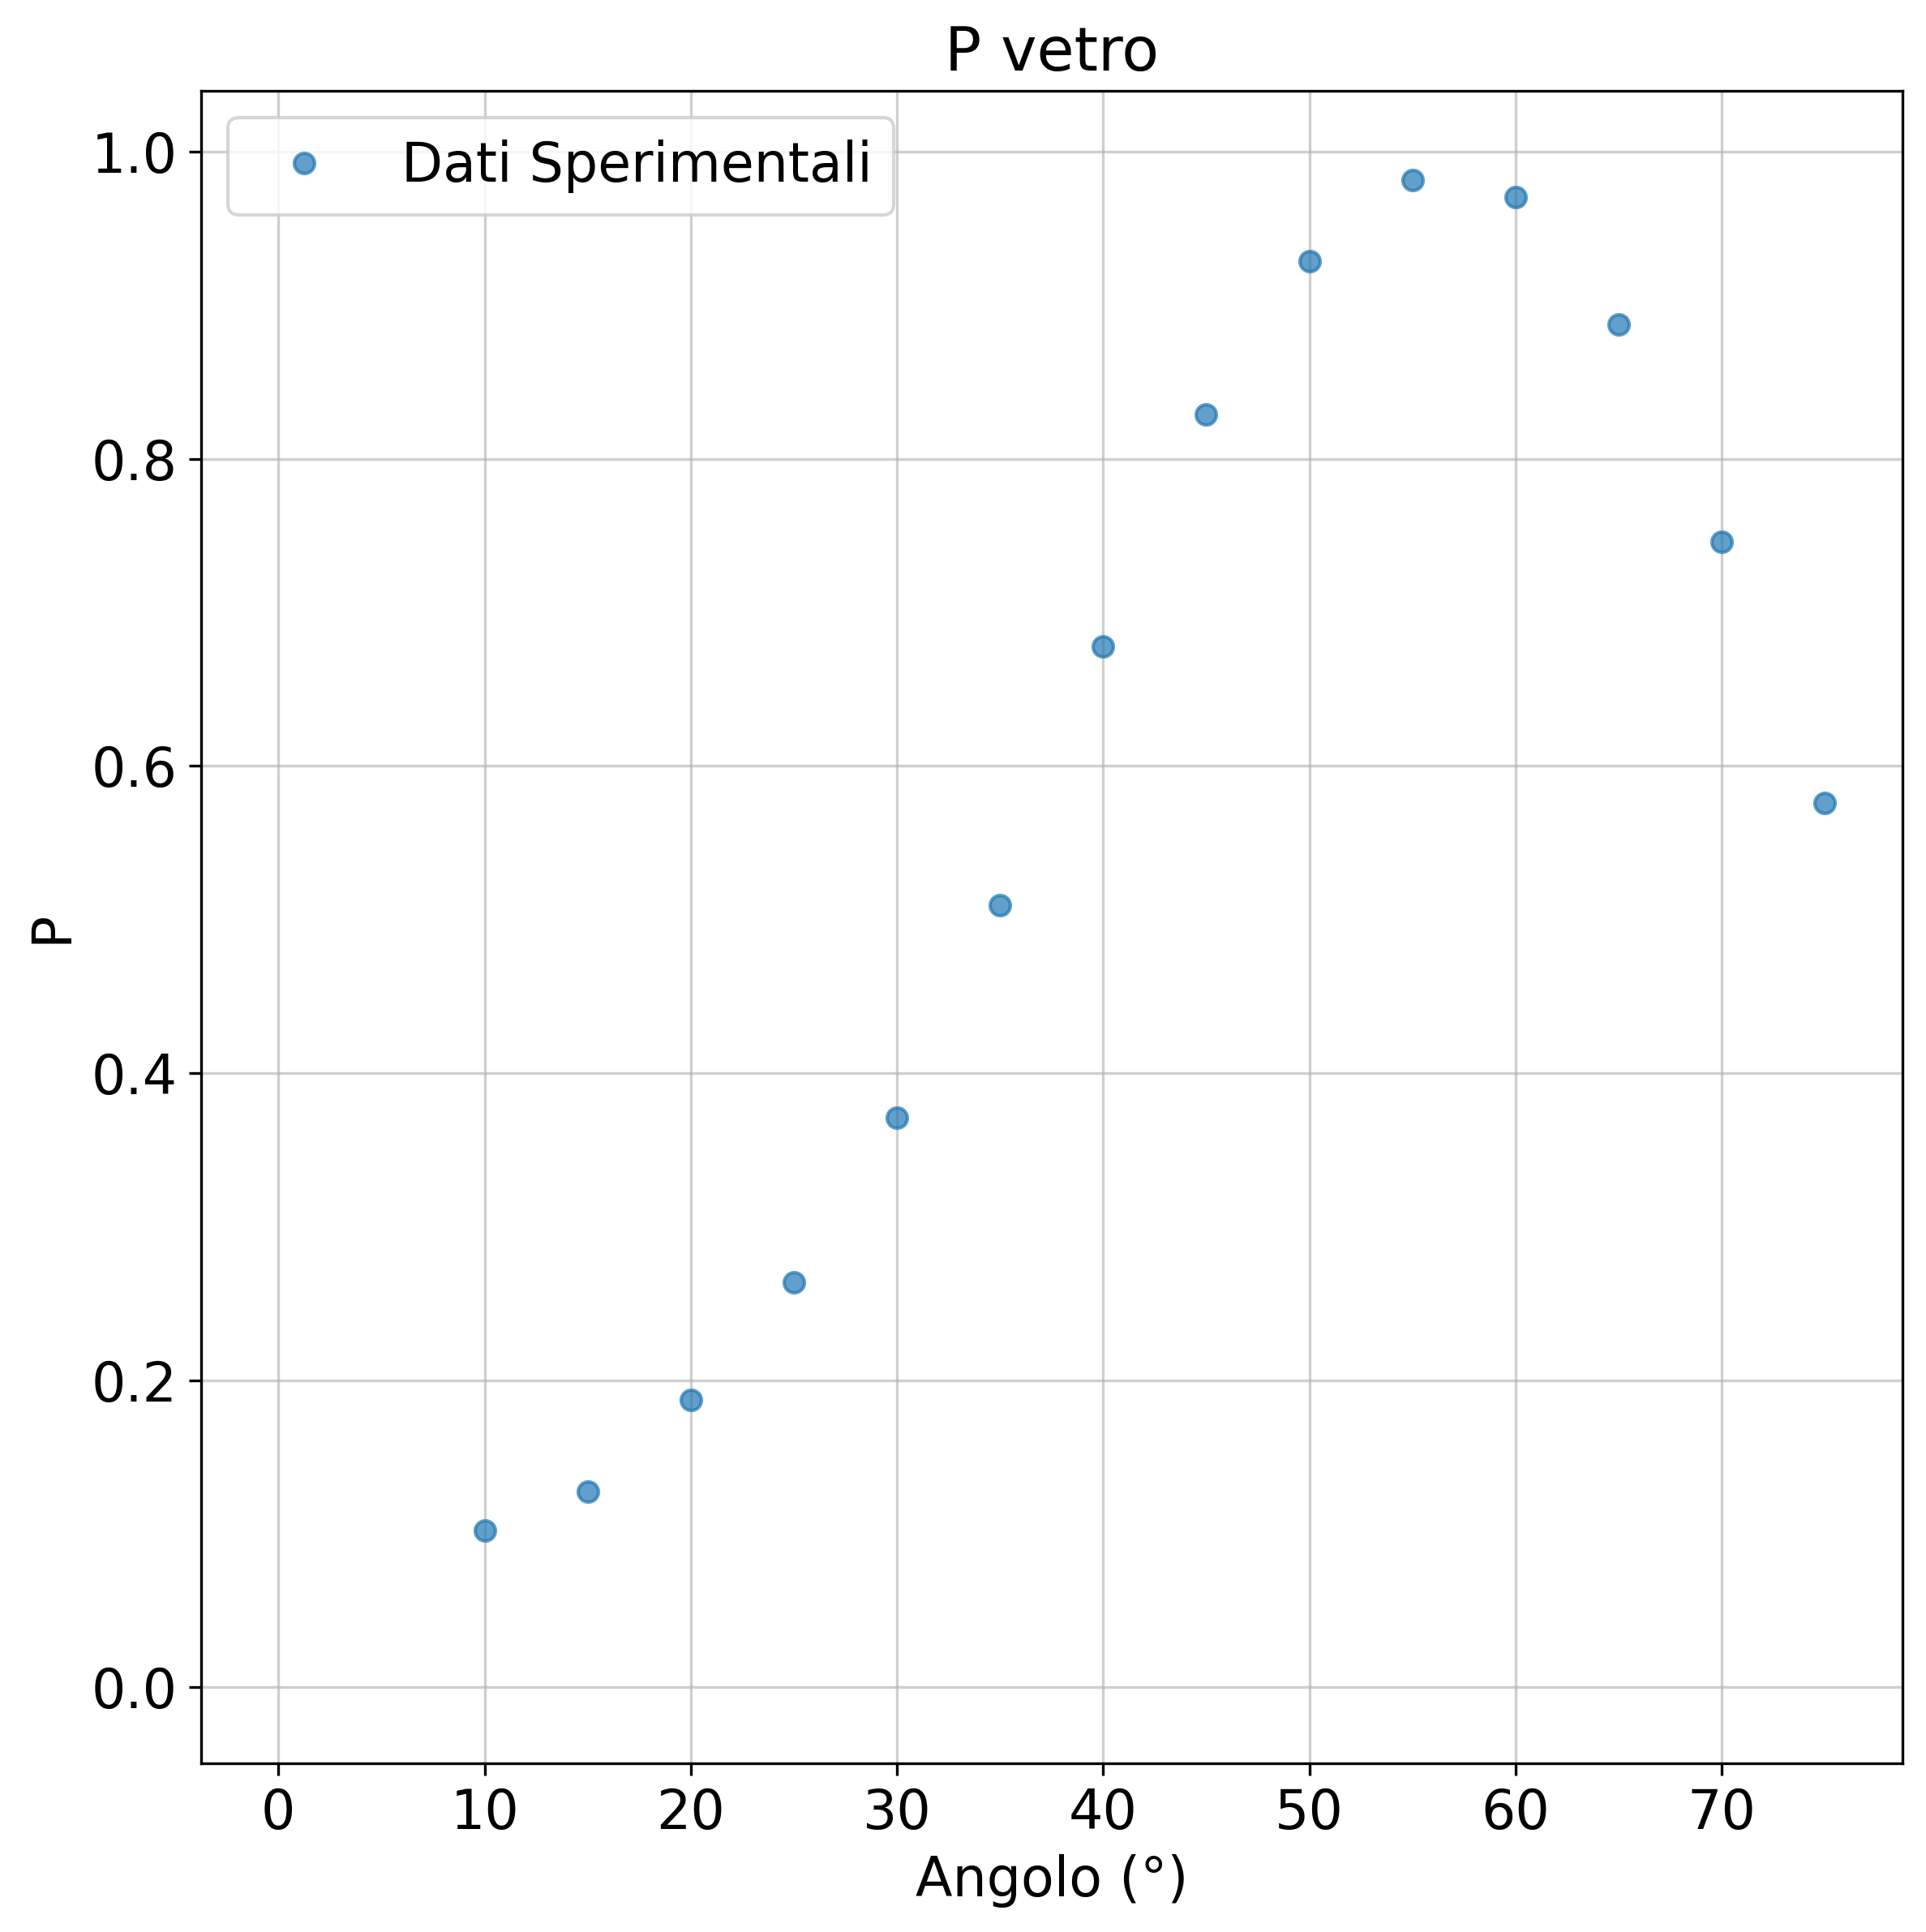
\includegraphics[width=\textwidth]{Dati_P vetro.png}
     \end{subfigure}
     \begin{subfigure}[b]{0.45\textwidth}
         \centering
         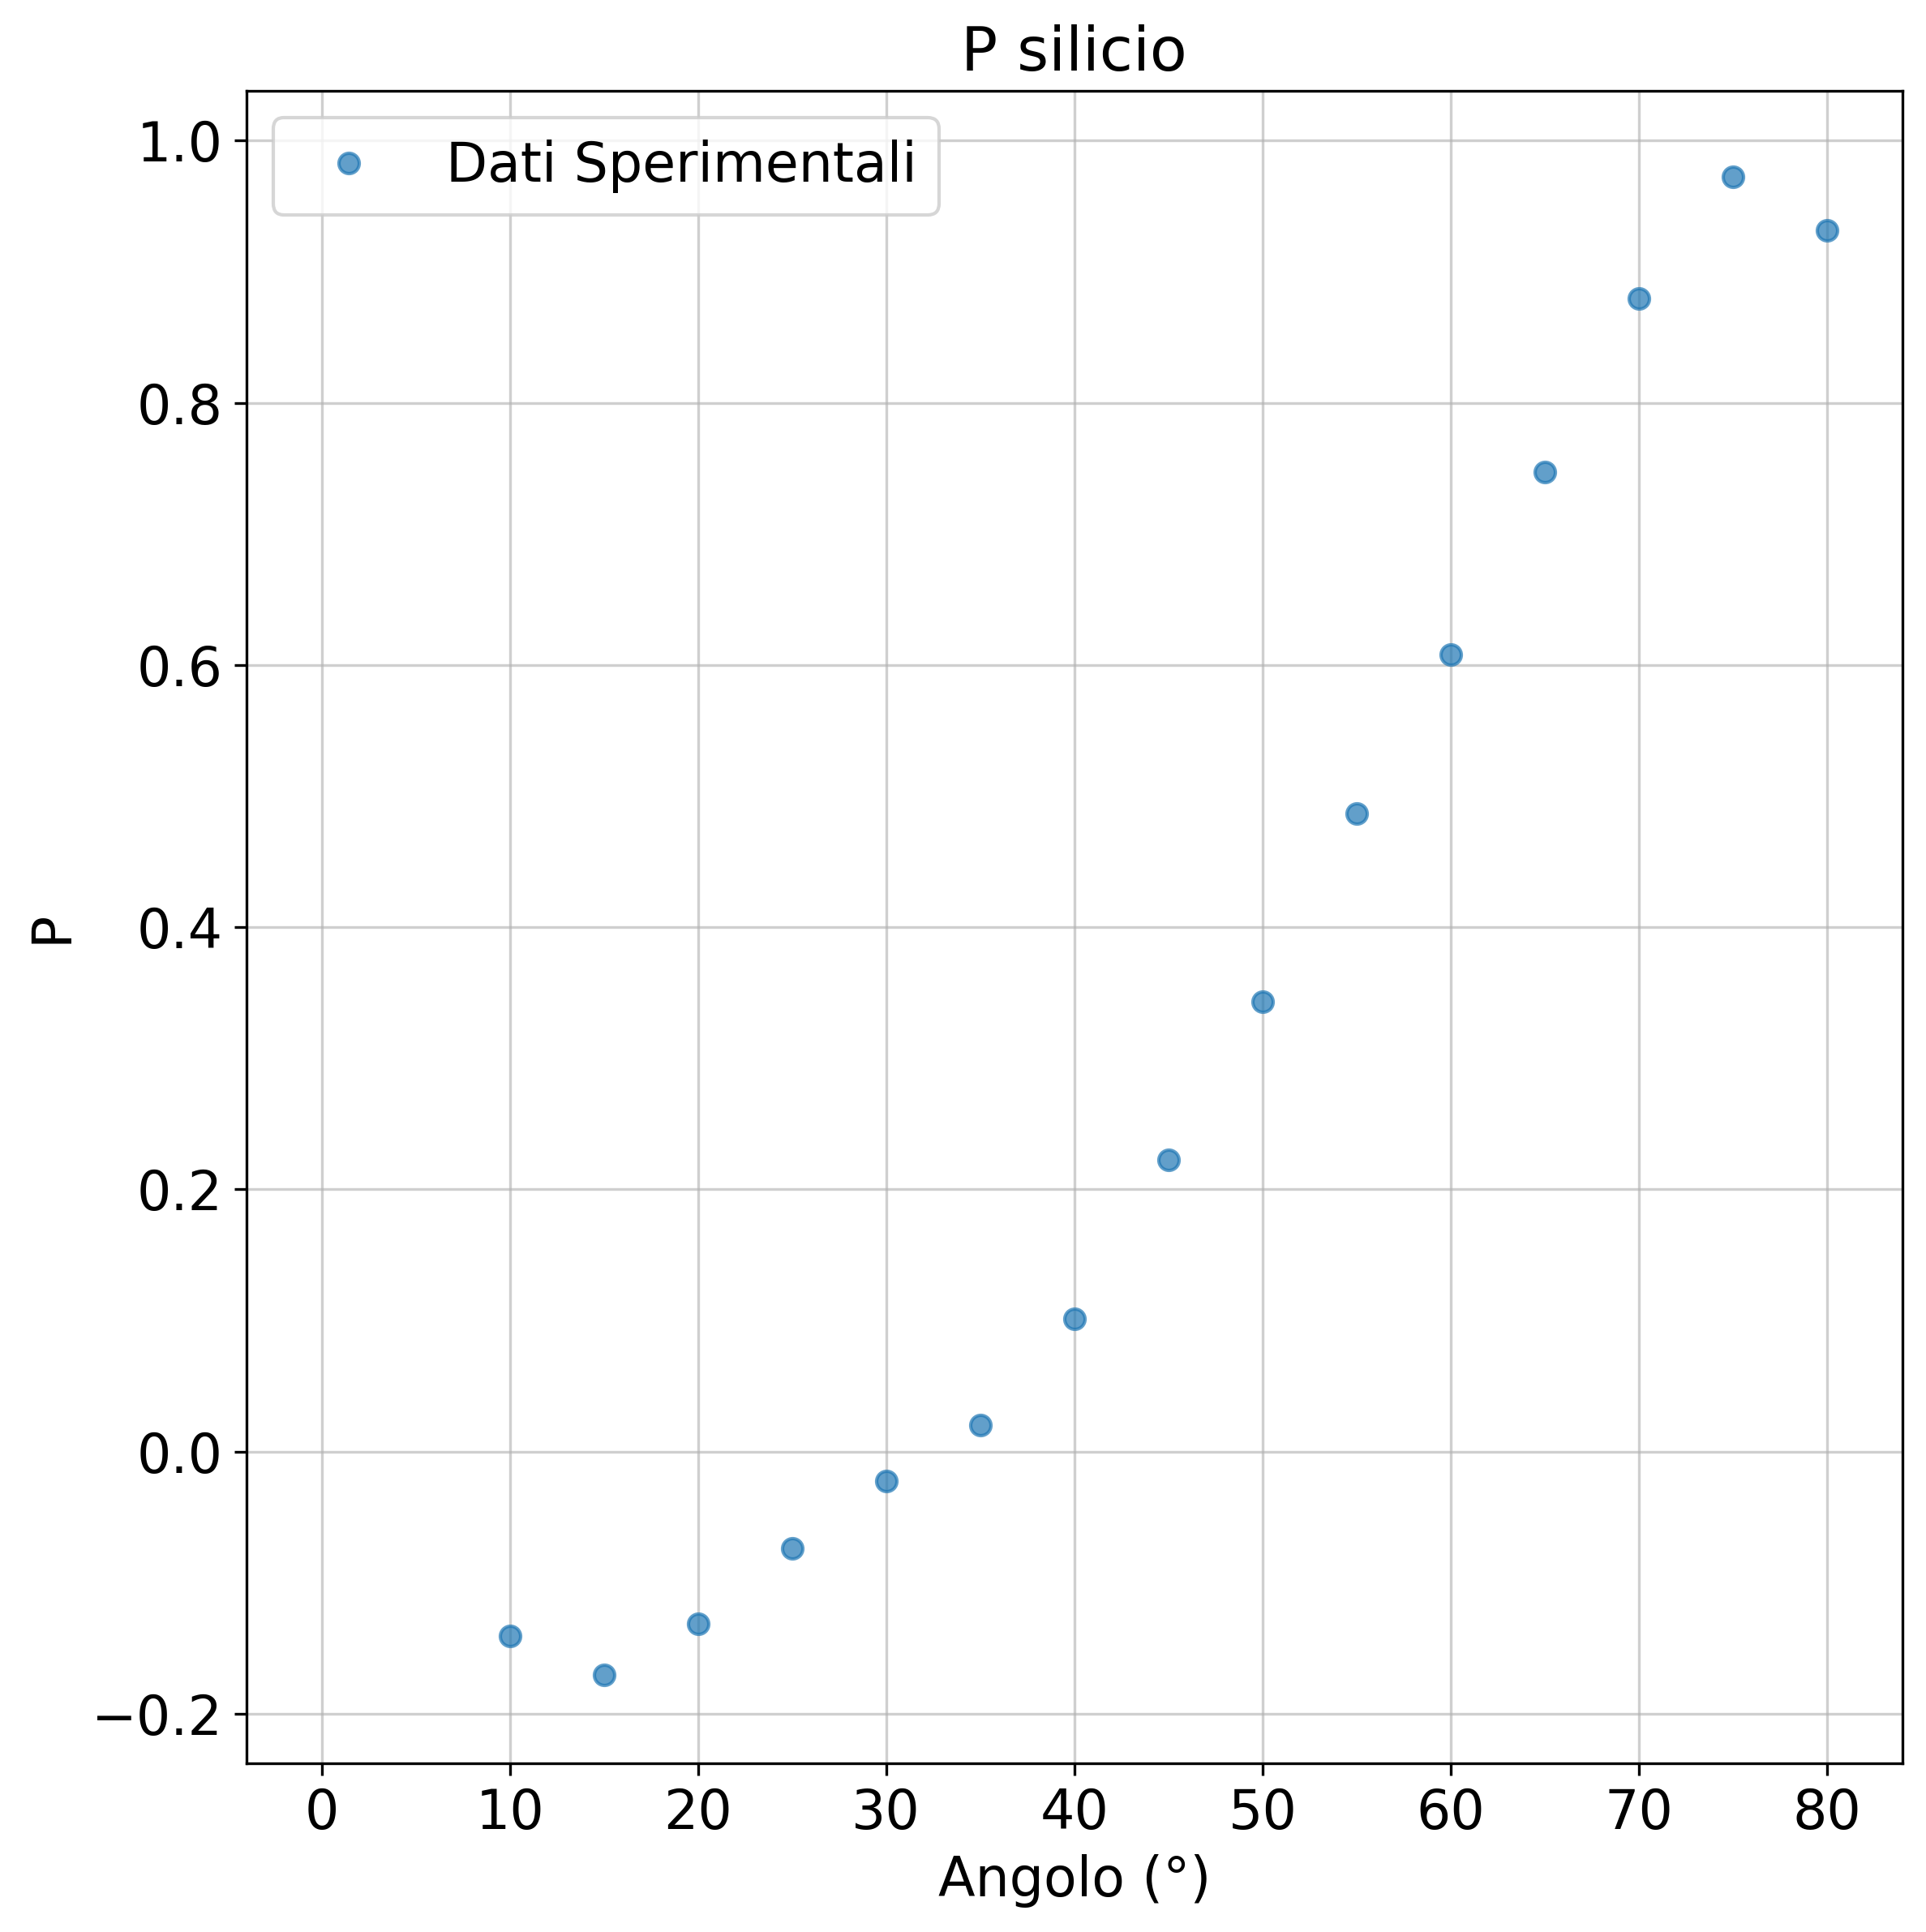
\includegraphics[width=\textwidth]{Dati_P silicio.png}
     \end{subfigure}
\end{figure}

Per quanto riguarda gli indici di rifrazione invece, sono stati restituiti come parametri dalla procedura di best-fit eseguita sulle distribuzioni angolari:

\begin{table}[H]
    \centering
    \begin{tabular}{
        l
        l
    }
        \toprule
        Campione & $n_{(525nm)}$ \\
        \midrule
        $SiO_2$ & $1.54\pm0.05$ \\
        $Si$ & $3.08\pm1.01$\\
        \bottomrule
    \end{tabular}
    \caption{Indici di rifrazioni ricavati tramite fit}
\end{table}

\section{Conclusioni}
Le distribuzioni angolari misurate seguono l'andamento teorico previsto. Per entrambi i materiali è nettamente visibile l'effetto dell'angolo di Brewster, il quale evidenzia la differente risposta ottica tra un mezzo trasmissivo, come $SiO_2$, ed uno riflettente/assorbente, come $Si$.
La misura di $\theta_B$ risulta in buon accordo con il valore atteso; inoltre, sfruttando la relazione $tan(\theta_B) = n(\lambda)$ si conferma la coerenza tra la stima qualitativa e i risultati ottenuti tramite la procedura di best-fit.
Per quanto concerne il grado di polarizzazione si osserva come il picco coincida con l'angolo di Brewster. Tuttavia, nel caso del silicio si registrano inizialmente valori negativi: ciò è verosimilmente imputabile alla difficoltà sperimentale di mantenere il campione perfettamente ortogonale rispetto al banco di lavoro.
Infine l'elevato errore relativo nella stima di $n(\lambda)$ per il silicio è probabilmente da attribuirsi alla difficoltà di eseguire il fit in presenza di una componente immaginaria dell'indice di rifrazione non nulla.
\end{document}
